\section{Echtzeitholographie}
\subsection{Versuchsbeschreibung}
Bei der Echtzeitholographie wird ein Hologramm aufgenommen und dieses mit dem Bild des Objektes überlagert. Unterschiede zwischen dem Objekt und seinem Hologramm können dann als Interferenzmuster beobachtet werden, solange sie nicht zu groß sind. In unserem Experiment wollen wir mit dieser Methode die resonanten Schwingungen einer 
\subsection{Durchführung und Auswertung}

\begin{figure}[ht]
 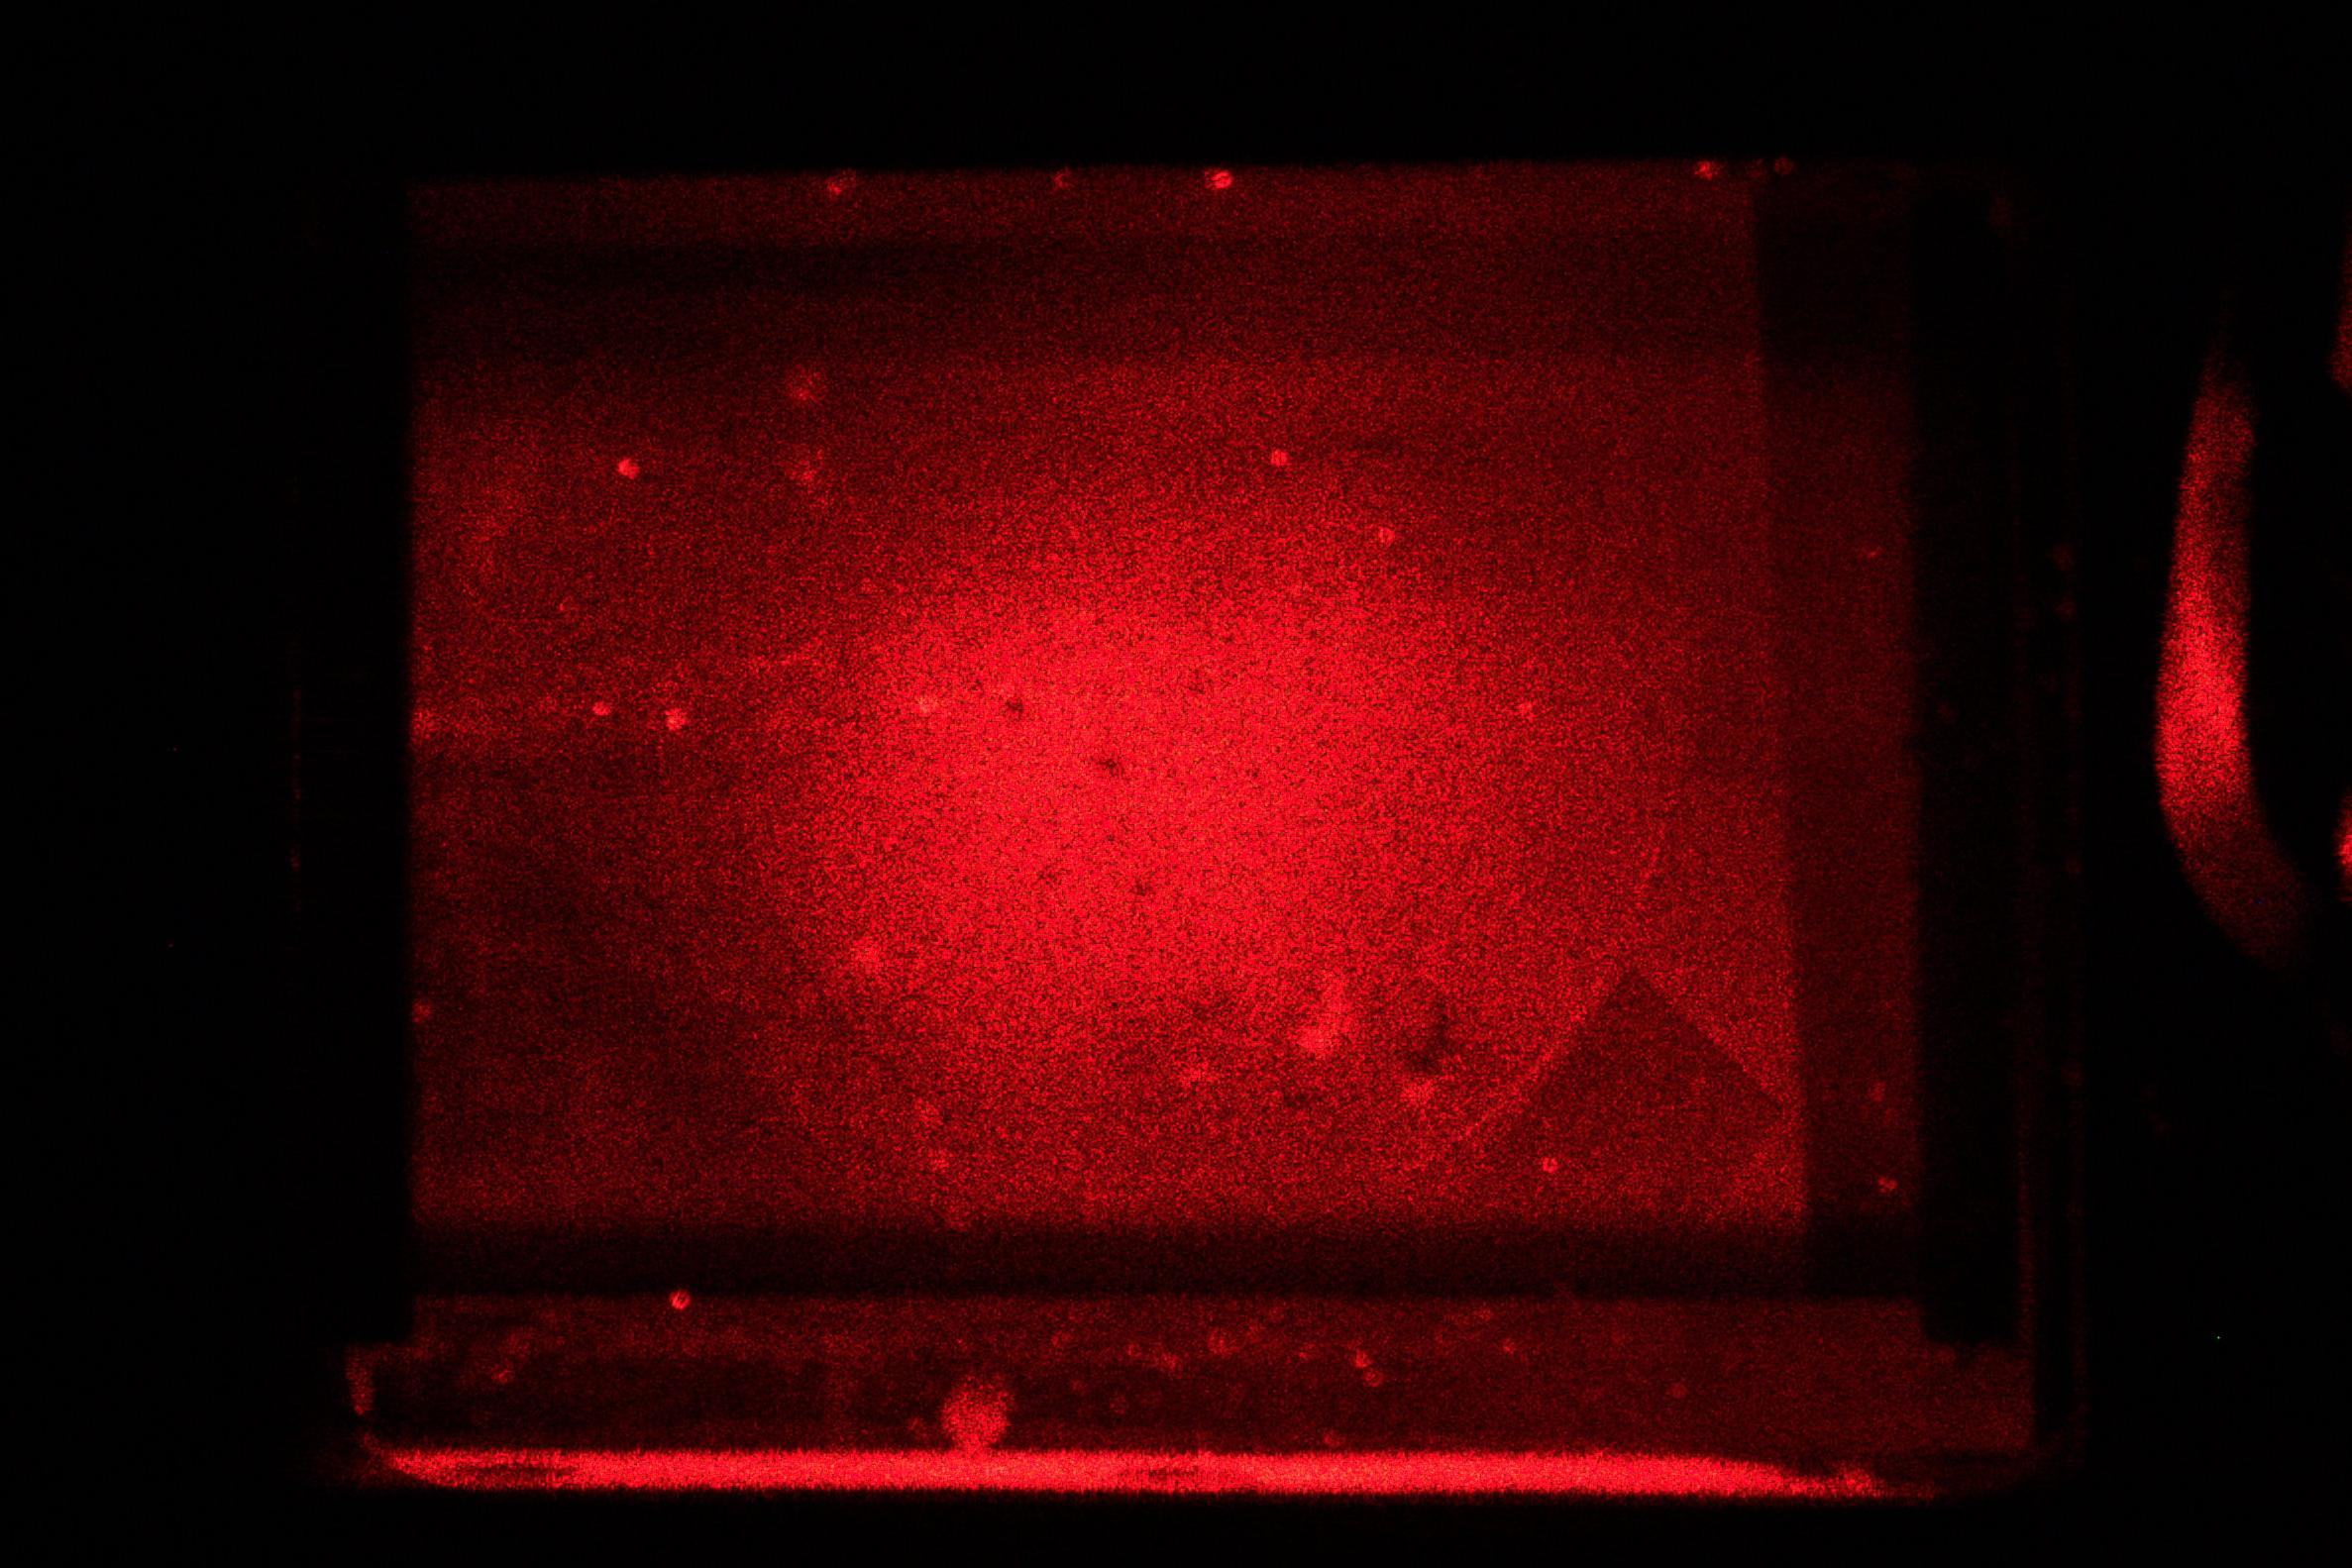
\includegraphics[width=\textwidth]{Photos/IMG_3927.jpg}
 \caption{Hologramm der Aluminiumplatte}
\end{figure}

